\documentclass[num-refs]{wiley-article}
\usepackage{graphicx} 
\usepackage{tikz}% Required for inserting images
%\usepackage[letterpaper,top=2.54cm,bottom=2.54cm,left=3.17cm,right=3.17cm,marginparwidth=1.75cm]{geometry}
\usepackage{hyperref}
\usepackage{setspace}
\usepackage{amsmath}
\usepackage[numbers]{natbib}


%\renewcommand{\includegraphics}[2][]{}

\papertype{Original Article}
% Include section in journal if known, otherwise delete
\paperfield{Journal Section}

\title{Practical Concerns for Estimating Mixed Hidden Markov Models with an Application to NHANES}
\abbrevs{PAM, physical activity monitor; PSG, polysomnography; HMM, hidden Markov model; MHMM, mixed hidden Markov model; NL, nested loop; RE, random effect.}

\author[1,2\authfn{1}]{Jordan Aron}
\author[1]{Paul S Albert}
\author[2]{Mark B Fiecas}
\affil[1]{Division of Cancer Epidemiology and Genetics, National Cancer Institute, Bethesda, Maryland, USA}
\affil[2]{Department of Biostatistics, University of Minneosta, Minneapolis, Minnesota, USA}
\corraddress{Jordan Aron of Division of Cancer Epidemiology and Genetics, National Cancer Institute, Bethesda, Maryland, USA and Department of Biostatistics, University of Minneosta, Minneapolis, Minnesota, USA}
\corremail{jordan.aron@nih.gov}


\begin{document}

\begin{frontmatter}
    \maketitle
    
    \begin{abstract}
    This is a generic template designed for use by multiple journals, which includes several options for customization. Please consult the author guidelines for the journal to which you are submitting in order to confirm that your manuscript will comply with the journal's requirements. Please replace this text with your abstract.
    
    % Please include a maximum of seven keywords
    \keywords{keyword 1, \emph{keyword 2}, keyword 3, keyword 4, keyword 5, keyword 6, keyword 7}
    \end{abstract}
\end{frontmatter}

\section{Introduction}

The circadian rhythm plays a wide-ranging role in human health, from regulating important metabolic pathways \cite{potterCircadianRhythmSleep2016} to immune response \cite{sharmaCircadianRhythmDisruption2016}. Disruption of the circadian rhythm is associated with a variety of negative health outcomes. For instance, sleep disruption related to shift work is most likely carcinogenic \cite{iarc2010}. Polysomnography (PSG) is the gold standard when evaluating certain sleep disorders, however PSG is both costly and inconvenient for patients\cite{chervin1999}. Requiring an overnight study at a heath care facility, there has been considerable interest in finding a cost-effective replacement that can amass population level data. 

The proliferation of personal physical activity monitors (PAM) offers an interesting insight into sleep health. Actigraphy has proven to be useful in assessing circadian rhythm disorders \cite{morgenthaler2007} and has some distinct advantages over PSG. PAMs collect a large amount of data over a longer period of time. As they are relatively inexpensive, more data can be collected on more people compared to PSG. Actigraphy has been, and continues to be, a popular way to study sleep \cite{ancoli-israelRoleActigraphyStudy2003,sadehRoleActigraphySleep2002,liguoriEvolvingRoleQuantitative2023}.

Although leveraging actigraphy data to study sleep is an exciting opportunity, there are challenges. PAMs measures movement, not sleep, and although there is a clear connection between the two, the specific relationship is difficult to ascertain. High activity periods most likely indicate an underlying wake state, however periods of inactivity may be hard to classify. Activity data may look similar for sedentary wake activities and sleep (e.g., watching TV may appear similar sleeping). In addition, there is often a large presence of zeros in the observed data due to very low activity. We propose to use an extension of a hidden Markov model (HMM) to capture this behavior. The observed data will be the activity measurements from the PAM and the Markov state will be the unobserved wake/sleep status.

In recent years HMMs have been applied numerous times to actigraphy data \cite{Liu2020a,Boeker2021} as they have been shown to be fairly accurate in classifying sleep and wake states \cite{Li2020,Witowski2014}. A constant (homogenous) transition matrix is used in many applications \cite{Xu2022,Su2022}, and although this leads to easier calculations, it does not account for the heterogeneity of wake/sleep times in the transition probabilities. Non-homogenous transition matrices have been used, however the sample size is often limited \cite{Ogbagaber2024,Huang2018a} as there is no closed form solution for estimating the transition probabilities. Heterogeneity is important to model as both sleep parameters and activity levels depend on a variety of factors \cite{etindele2022,Salvo2015,mitchell2017}. 

Physical activity is not uniform among the US population \cite{hootman2003} and this person-to-person variability must be accounted for in any HMM. Previously this issue has been handled by estimating individual level parameters, however as the number of participants increases so too does the number of parameters. This approach is feasible for numerous repeated measurements collected per person. Another approach extends the Markov state space from wake and sleep to high activity, low activity, and rest \cite{Huang2018a,Boeker2021}. This solution may cause more problems than it solves as it complicates the interpretation of the latent states. Additionally, this increases the complexity of adding important covariates to the Markov transition matrix. Estimating a $3\times3$ transition matrix is much more difficult than a $2\cdot2$, causing feasibility issues when large amounts of data are used. 

We propose a mixed HMM (MHMM) \cite{altmanMixedHiddenMarkov2007, maruotti2009,maruottiMixedHiddenMarkov2011} with an individual level random effect (RE) for the activity data in the wake state and a non-homogenous transition matrix with additional age covariates. A MHMM for actigraphy data has been proposed before, however the RE was in the latent transition process \cite{Duroy2020}. The RE in the emission distribution allows people to have different levels of activity while keeping the interpretable and computation friendly two state structure. We use a non-parametric approach to estimate the heterogeneity in the emission distribution as there is little precedent on how activity is distributed across the US population.

As a MHMM with a RE in the emission distribution has not been applied to actigraphy data previously, it is not clear whether it confers any advantage over standard HMMs. In general, the situations where a MHMM with a RE in the emission distribution outperforms a HMM with individual emission parameters have not been extensively studied before. Akin to the investigation by McClintock \cite{mcclintock2021}, we provide an in-depth simulation study to determine the usefulness of a MHMM in this setting. Specifically, we aim to answer whether a MHMM is beneficial for state reconstruction, or if a HMM is sufficient. Additionally, we give recommendations for nonparametric density estimation for the MHMM emission distribution RE. Afterwards we apply a standard HMM and MHMM to National Health Examination Survey physical activity data.

\section{Methods} \label{Methods}
\subsection{Notation}

Define the set $\{S_{i1}, ..., S_{iT}\}$ as the states of a first order Markov chain (MC) corresponding to the sleep-wake cycle. If person $i$ at time $t$ is awake then $S_{it}=0$, if person $i$ is asleep at time $t$ then $S_{it}=1$. This first order MC can be completely described by an initial probability, $p_j=P(S_{i1} =j)$, and a (possibly non-homogenous) transition array, $\mathbf{P}(t)$.  Let entry $kj$ of $\mathbf{P}(t)$ be equal to $p_{kj}(it)=P(S_{it}=j|S_{it-1}=k)$. To allow for covariates in the transition probabilities, we model the probability of changing states with the inverse logit function. We have $p_{01}(it) = \text{expit}(X_{it}\beta_0)$ and $p_{10}(it) = \text{expit}(X_{it}\beta_1)$ where $X_{it}$ is a vector of covariates and $\beta_j$ is the corresponding vector of covariate parameters. This allows both fixed (e.g., race) and time-varying (e.g., current time) covariates to influence the transition probabilities.

Define the set $\{a_{i1}, ..., a_{iT}\}$ as the observed physical activity data from a PAM for patient $i$. For person $i$ at time $t$, we refer to the distribution of the activity measurement given the current wake/sleep state as the emission distribution. To account for semicontinuous data, we assume that the emission distribution is characterized with a mass at zero and the normal distribution when non-zero. When $S_{it}=1$, we assume $a_{it} = 0$ with probability $\lambda_1$. With probability $1-\lambda_1$ we assume $a_{it}$ is drawn from a normal distribution centered at $\mu_1$ with variance $\sigma_1^2$. When $S_{it}=0$, we assume $a_{it} = 0$ with probability $\lambda_0$. With probability $1 - \lambda_0$ we assume $a_{it}$ is drawn from a normal distribution centered at $\mu_0+u_i$ with variance $\sigma_0^2$, where $u_i$ as an individual random effect directly related to the mean wake activity of person i. We impose no restrictions on the continuous distribution for $u_i$, call it H. We refer to the HMM with a RE in the emission distribution as a mixed HMM (MHMM). The current activity measurement ($a_{it}$) given the current sleep status is independent of all other MC states, or equivalently $P(a_{it}|S_{i1}, ..., S_{iT}) = P(a_{it}|S_{it})$. Therefore, the MHMM can be completely described by the initial, transition, and emission probabilities.
 
\subsection{Estimation}

Without applying any additional techniques, the likelihood is 

\begin{equation*}
f(\textbf{a}|\theta) = \prod_{i=1}^n \int_U \sum_{{s_1}\cdots{s_T}} \biggr[ 
    p_{s_1} \prod_{t=2}^T p_{s_{t-1}s_t}(it) \prod_{t=1}^T \lambda_{s_t}^{\delta_{it}} \big[(1-\lambda_{s_t})P(a_{it}|S_{it}=s_t,u_i)\big]^{1-\delta_{it}}\biggr] dH(u_i),
\end{equation*}
where $\theta$ is the collection of all parameters. As we do not know the underlying MC state, it is not clear yet how to calculate these probabilities as the wake/sleep states are not observed. As $u_i$ is a continuous individual level random effect, we must integrate over its support for each individual. This integral is complex and requires numerical methods to solve. The next two subsections will detail how to calculate this likelihood. 



\subsubsection{Nonparametric Density Estimation (NPDE)}

To simplify the integral (as well as allowing future computations with the forward-backward algorithm), we will estimate the continuous RE distribution, H, with a discrete random variable, $b_i$. A few support points are chosen where the mass put on support point $l$ is $\pi_l$. This can equivalently be written as $P(b_i = r_l) = \pi_l$ where $r_l$ is support point l. Conceptually, this can be thought of as estimating a discrete distribution using a histogram where each bar of the histogram is a support point and the mass put on each support point is the height of the bar. Using one support point is equivalent to leaving out the RE and thus the MHMM reduces to a HMM with shared emission parameters. Using NPDE we can write the likelihood as follows: 

\begin{equation*}\label{like2}
    \begin{split}
f(\textbf{a}|\theta) = \prod_{i=1}^n \sum_{l=1}^L \sum_{{s_1}\cdots{s_T}} \biggr[ 
    p_{s_1} & \prod_{t=2}^T p_{s_{t-1}s_t}(it) 
    \prod_{t=1}^T \lambda_{s_t}^{\delta_{it}} \big[(1-\lambda_{s_t})P(a_{it}|S_{it}=s_t,b_i=r_l)\big]^{1-\delta_{it}} \biggr] \pi_l,
    \end{split}
\end{equation*}
where we sum over the number of support points, L, instead of integrating over the support of U. Thus, the time needed to compute this likelihood scales linearly with L. Increasing L increases estimation accuracy, however it comes at a computational price. L must be chosen before estimation, and we will discuss how to choose this number based on results from our simulation study in Section \ref{SimStudy}.

\subsubsection{EM Algorithm Overview}

The EM algorithm is an iterative technique to perform maximum likelihood estimation in the presence of latent variables \cite{dempster1977}. Each iteration of the algorithm alternates between an expectation (E) and maximization (M) step, where the likelihood increases each iteration. Once this increase becomes sufficiently small, we consider the algorithm converged and stop. For the E step, we calculate the expected value of the full data log likelihood conditional on the observed data. We then maximize this expectation in the M step. The complete data likelihood, written down as if we knew the latent variables that are required for estimation, is: 

\begin{equation}\label{cdata}
\begin{split}
    f(\textbf{a},\textbf{S}, \textbf{b} | \theta)  = & \prod_{i=1}^n \prod_{j=0}^1 
        b_j^{I(S_{i1}=j)} \times \\
    & \prod_{i=1}^n \prod^T_{t=2} \prod_{k=0}^1 \prod_{j=0}^1  
        b_{kj}(it)^{I(S_{it-1}=k,S_{t}=j)} \times \\ 
    & \prod_{i=1}^n\prod_{l=1}^L \prod^T_{t=1}\prod_{j=0}^1 \biggr[
        \lambda_j^{\delta_{ij}} \big[(1-\lambda_j)P(a_{it}|S_{it}=j,b_i=r_l)\big]^{1-\delta_{ij}}
        \biggr]^{I(S_{it}=j,b_i=r_l)} \times\\
    & \prod_{i=1}^n\prod_{l=1}^L \pi_l^{I(b_i=r_l)},
\end{split}
\end{equation}
where I() is an indicator variable equal to 1 of the inside expression is true and 0 otherwise. We then take the expected value of the log of equation \ref{cdata}, conditioning on the observed data. The result is the expectation of the complete data log likelihood. The E step is computed as 
\begin{equation*}\label{ecdata}
\begin{split}
    \ell = & E\big[\text{log f}(\textbf{a},\textbf{S}, \textbf{b} | \theta) | \textbf{a},\theta\big]\\
    = & \sum_{i=1}^n\sum_{j=0}^1P(S_{i1}=j|\textbf{a})\text{log }b_j + \\
    & \sum_{i=1}^n \sum^T_{t=2} \sum_{k=0}^1 \sum_{j=0}^1 
        P(S_{it-1}=k,S_{it}=j|\textbf{a})\text{log }b_{kj}(it) + \\ 
    & \sum_{i=1}^n \sum_{l=1}^L \sum^T_{t=1}\sum_{j=0}^1 P(S_{it}=j,b_i=r_l|\textbf{a}) \biggr[
        \delta_{it}\text{log }\lambda_j + 
        (1-\delta_{ij})\text{log}\Big((1-\lambda_j)P(a_{t}|S_{it}=j, b_i=r_l) \Big)\biggr]+ \\
    &  \sum_{i=1}^n \sum_{l=1}^L P(b_i=r_l|\textbf{a}) \text{log }\pi_l .
\end{split}
\end{equation*}
To calculate this, we use a modified version of the forward-backward algorithm, detailed in the next section.

\subsubsection{E Step}
To account for the random effect in the emission distribution we use a modified version of the forward-backward algorithm that conditions on the discrete RE for person $i$ \cite{maruottiMixedHiddenMarkov2011}. The forward and backward quantities are $\alpha_{it}(j,r_l) = P(a_{i1}, ..., a_{it}, S_{it} = j | b_i=r_l)$ and $\beta_{it}(j,r_l) =  P(a_{it+1}, ..., a_{iT} | S_{it} = j,b_i=r_l)$, respectively. These quantities are calculated as: 
 
\begin{equation} \label{fwd}
    \alpha_{it}(j,r_l) = \begin{cases}
        p_{j} f(a_{i1}|S_{i1}=j,r_l) & \text{if } t = 1 \\
        \sum_{k=0}^1 \alpha_{it-1} (k,b_l)p_{kj}(it)\lambda_j^{\delta_{ij}} \big[(1-\lambda_j)P(a_{it}|S_{it}=j,b_i=r_l)\big]^{1-\delta_{ij}}
            & \text{if } t > 1\\
    \end{cases}
\end{equation}
and
    
\begin{equation} \label{bkwd}
\beta_{it}(j,r_l) = \begin{cases} 
    \sum_{k=0}^1p_{jk}(it)\lambda_j^{\delta_{ij}} \big[(1-\lambda_j)P(a_{it}|S_{it}=j,b_i=r_l)\big]^{1-\delta_{ij}}\beta_{it+1}(k,r_l) 
        & \text{if } t < n \\
    1 & \text{if } t = n. \\
\end{cases}
\end{equation}
Using the forward-backward algorithm we can now calculate the necessary components (equations \ref{proba}-\ref{probstran}) for the M step. 


\begin{equation}\label{proba}
\begin{split}
    P(\textbf{a}) & = \prod_{i=1}^n \sum_{l=1}^L 
        P(\textbf{a}|b_{i}=r_l)P(b_{i}=r_l) = 
    \prod_{i=1}^n \sum_{l=1}^L \sum_{j=0}^1 \alpha_{iT}(j,r_l)\pi_l 
\end{split}
\end{equation}

\begin{equation}\label{probl}
\begin{split}
    P(b_{i}=r_l|\textbf{a}) & = \frac{P(\textbf{a}|b_{i}=r_l)P(b_{i}=r_l)}{P(\textbf{a})} = 
    \frac{\sum_{j=0}^1 \alpha_{iT}(j,r_l)\pi_l }{P(\textbf{a})}  
\end{split}
\end{equation}

\begin{equation}\label{probs0}
\begin{split}
    P(S_{it}=0,b_{i}=r_l|\textbf{a}) = \frac{P(S_{it}=0,\textbf{a}|b_{i}=r_l)
        P(b_{i}=r_l)}{P(\textbf{a})} = 
    \frac{\alpha_{it}(0,r_l)\beta_{it}(0,r_l)\pi_l }{P(\textbf{a})} 
\end{split}
\end{equation}

\begin{equation}\label{probs1}
\begin{split}
    P(S_{it}=1|\textbf{a}) = 
    \frac{\sum^L_{l=1}P(S_{it}=1,\textbf{a}|b_{i}=r_l)
        P(b_{i}=r_l)}{P(\textbf{a})} = 
    \frac{\sum^L_{l=1}\alpha_{it}(1,r_l)\beta_{it}(1,r_l)\pi_l }{P(\textbf{a})} 
\end{split}
\end{equation}


\begin{equation}\label{probstran}
\begin{split}
    P(S_{it-1}=k,S_{it}=j|\textbf{a}) & = 
        \frac{P(S_{it-1}=k,S_{it}=j,\textbf{a})}{P(\textbf{a})} \\
    & = \frac{\sum^L_{l=1}\alpha_{it}(k,r_l) p_{kj} P(a_{it}|S_{it}=j, b_i=r_l)
        \beta_{it}(j,r_l)\pi_l }{P(\textbf{a})} 
\end{split}
\end{equation}



\subsubsection{M Step}

 To maximize with respect to each parameter, we set the derivative of the likelihood with respect to that parameter to 0 and solve. This approach has a modular nature as the initial, transition, emission, and mixing ($\pi_l$) probabilities can be optimized independently. Using the previously described adapted forward-backward algorithm, we can calculate closed form solutions for the initial, emission, and mixing parameters (equations \ref{init}-\ref{pi}). As we cannot observe $\mu_0$ or $r_l$ individually, we cannot estimate either independently. This does not create a problem as the sum of the two quantities is the necessary component for the model and can be estimated. We will refer to $\nu_l$ as the cluster mean in future sections. 

\begin{equation}\label{init}
    \hat{p}_j  = \frac{\sum^n_{i=0} P(S_{i1}=0|\textbf{a})}{n}
\end{equation} 

\begin{equation}\label{binom}
    \hat{\lambda}_j  = \frac{\sum^n_{i=0} \sum_{t=1}^T P(S_{it}=j|\textbf{a})\delta_{it}}
                            {\sum^n_{i=0} \sum_{t=1}^TP(S_{it}=j|\textbf{a})}
\end{equation} 

\begin{equation}\label{mu0}
    \hat{\mu}_0 + \hat{r}_l = \hat{\nu}_l = 
    \frac{\sum_{i=1}^n \sum_{t=1}^T (1-\delta_{it})a_{it}P(S_{it}=0,b_{i}=r_l|\textbf{a})}
    {\sum_{i=1}^n \sum_{t=1}^T (1-\delta_{it})P(S_{it}=0,b_{i}=r_l|\textbf{a})}
\end{equation} 

\begin{equation}\label{sig0}
    \hat{\sigma}_0^2 = 
    \frac{\sum_{i=1}^n \sum_{l=1}^L \sum_{t=1}^T (1-\delta_{it})(a_{it}-\nu_l)^2 P(S_{it}=0,b_{i}=r_l|\textbf{a})}
        {\sum_{i=1}^n \sum_{l=1}^L \sum_{t=1}^T (1-\delta_{it}) P(S_{it}=0,b_{i}=r_l|\textbf{a})}
\end{equation} 

\begin{equation}\label{mu1}
    \hat{\mu}_1 = 
    \frac{\sum_{i=1}^n \sum_{t=1}^T a_{it}(1-\delta_{it})P(S_{it}=1|\textbf{a})}
        {\sum_{i=1}^n \sum_{t=1}^T (1-\delta_{it})P(S_{it}=1|\textbf{a})}
\end{equation} 

\begin{equation}\label{sig1}
    \hat{\sigma}_1^2 = 
    \frac{\sum_{i=1}^n \sum_{l=1}^L \sum_{t=1}^T (1-\delta_{it})(a_{it}-\mu_1)^2 P(S_{it}=1|\textbf{a})}
        {\sum_{i=1}^n \sum_{l=1}^L \sum_{t=1}^T (1-\delta_{it}) P(S_{it}=1|\textbf{a})}
\end{equation} 

\begin{equation}\label{pi}
    \hat{\pi}_l = \sum_{i = 1}^n \frac{P(b_i = r_l)}{n}
\end{equation}


Unlike the previous parameters, no closed form solution exists for the transition probabilities. Instead, we perform a single Newton-Raphson step at each iteration of the EM algorithm. Performing multiple Newton-Raphson steps in each iteration drastically increases the computational time. As the EM algorithm is iterative, multiple steps of the Newton-Raphson are calculated before convergence. This technique has similar convergence properties to maximum likelihood estimation for large datasets \cite{brousteOneStepCamOnestep2021}. We have not observed non-monotonicity of the likelihood with this approach. Thus, $\beta_{j}^* = \beta_{j} - (\frac{\partial^2\ell}{\partial \beta_{j}^2})^{-1} \frac{\partial\ell}{\partial \beta_{j}}$, where $\beta_{j}$ is our current estimate and $\beta_{j}^*$ is our updated estimate. 

\section{Simulation Study}\label{SimStudy}

\subsection{Simulation Settings} \label{SimSettings}

The following two questions motivated this simulation study. Do MHMMs provide enough of an advantage to motivate their use compared to standard HMMs? When estimating a MHMM how many support points are necessary for the NPDE of the RE distribution? Three different types of HMMs were tested: HMM where each person has their own wake activity mean and variance parameter (individual HMM), HMM where there is a shared wake activity mean and variance parameter (shared HMM), and seven MHMMs with two to eight support points (MHMM2-MHMM8) as described by section \ref{Methods}. The shared HMM is a special case of a MHMM with one support point. For all models, the initial, transition, and sleep emission parameters are shared across all individuals.

We first simulate the sequence of MC states corresponding to the wake/sleep state of person $i$ at time $t$ according to pre-specified initial and transition probabilities. For the transition probabilities, we let $\beta_j = \{\beta_{j0}, ..., \beta_{j8}\}$ and $X_{it} = \{1, x_{it1}, ..., x_{it8}\}$, where:
\begin{itemize}
    \item $x_{it1}$ and $x_{it2}$ are fixed covariates equal to 1 if that covariate applies to person i.
    \item $x_{it3} = \text{cos}(\frac{2\pi t}{96})$ and $x_{it4} = \text{sin}(\frac{2\pi t}{96})$ vary by time to account for the circadian rhythm.
    \item $x_{it5}$ and $x_{it6}$ are the respective cosine and sine terms for the first fixed covariate.
    \item $x_{it7}$ and $x_{it8}$ are the respective cosine and sine terms for the second fixed covariate.
\end{itemize}

Any first order harmonic function with a period of 96 can be estimated. A period of 96 was chosen as this is equivalent to dividing each day into 15 minute intervals. We vary both the number of people (1000 and 5000) and the length observations per person (one day and one week of follow up). For each person, we draw $u_i$ from H. We considered different underlying RE distribution such that H is Normal, Gamma, Normal/Gamma mixture, and t with 3 degrees of freedom (Figure \ref{REdist}). We then simulate the observed activity data where $a_{it} \sim N(2+u_i,1)$ if $S_{it}=0$ and $a_{it} \sim N(0,2)$ if $S_{it}=1$ and estimate the model parameters using each of the different types of HMMs. Lastly, we use the Viterbi algorithm to construct the most likely sequence of the latent wake/sleep states given our estimated parameters. We compare the estimated sequence with the true wake/sleep sequence. This was repeated 100 times for each combination (model, number of people, length of observation, choice of H).


\subsection{Results}\label{SimStudyResults}

\begin{figure}
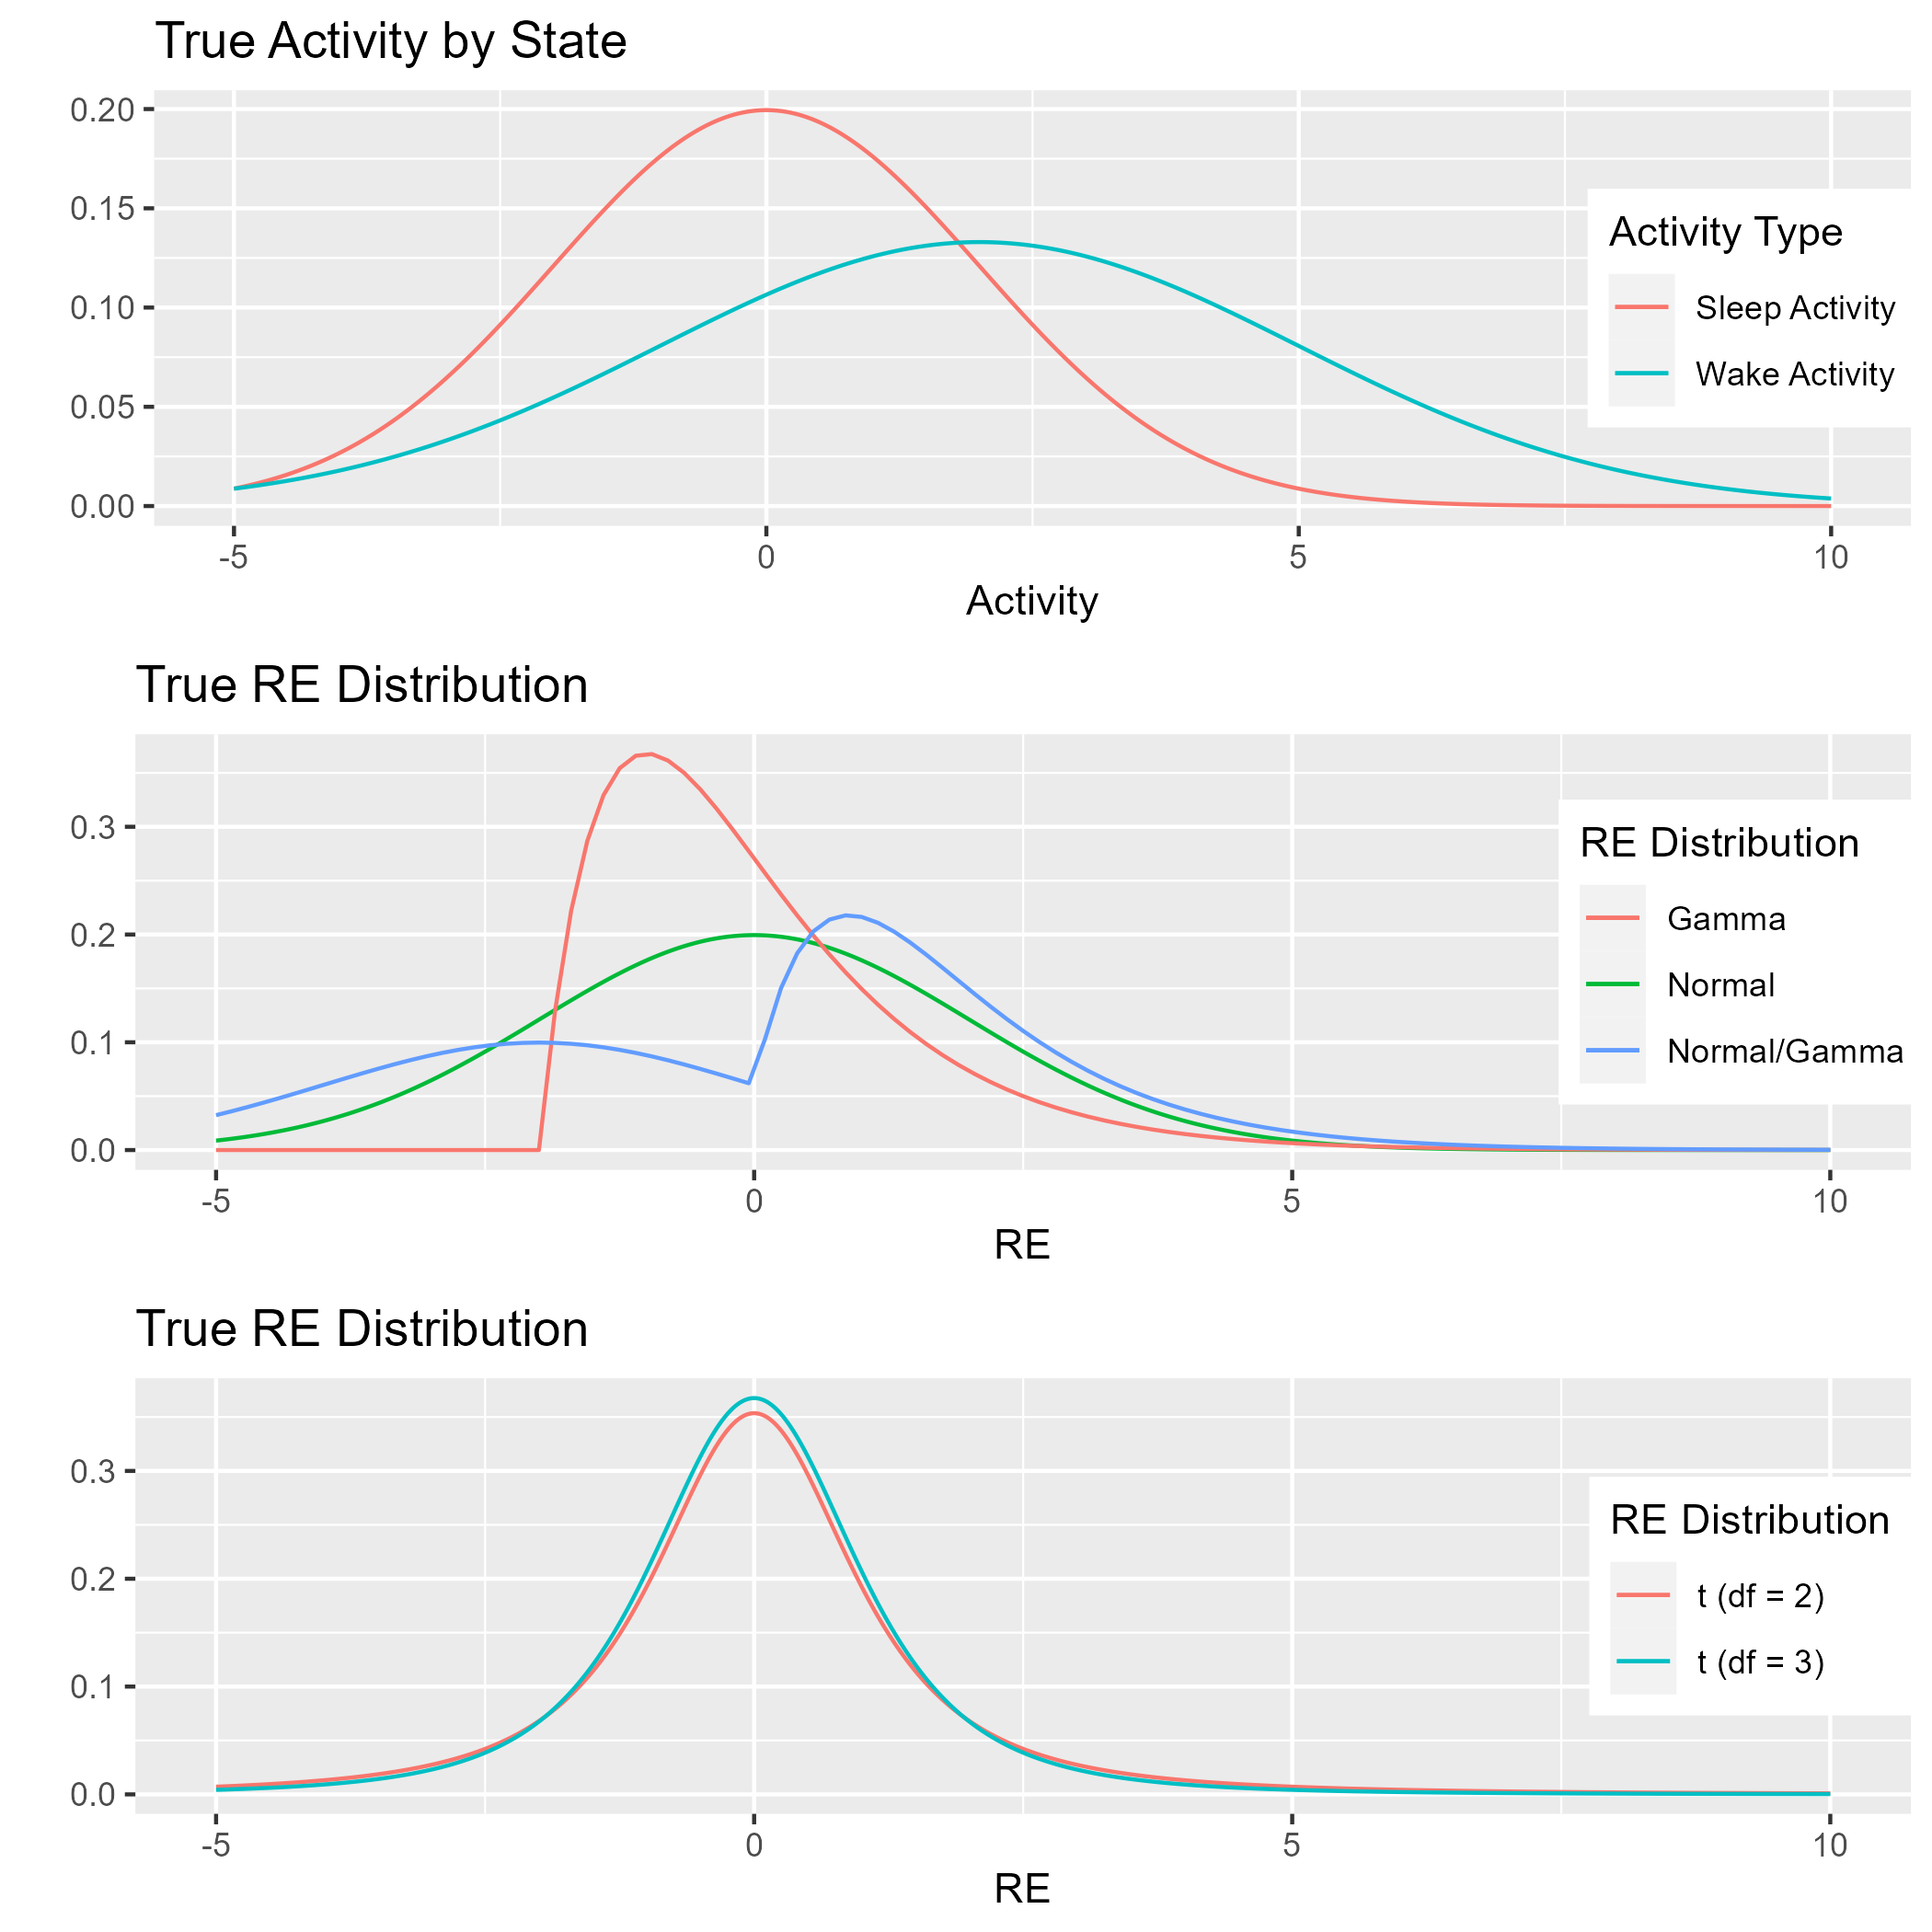
\includegraphics[scale=.5]{Support/REdist.png}
\centering
\caption{Top plot shows wake (without RE) and sleep activity distribution. Bottom plot shows the possible choices for H, the continuous RE distribution.}
\label{REdist}
\end{figure}

The top plot of figure \ref{REdist} shows the wake (without a RE) and sleep activity distribution. Each individual's wake activity distribution is shifted to the right or left depending on $u_i$. The bottom plot shows the different choices for H. We center H around 0 so that the expected overlap between the wake and sleep activity distributions is the same for each person for all choices of H. 

\begin{figure}
    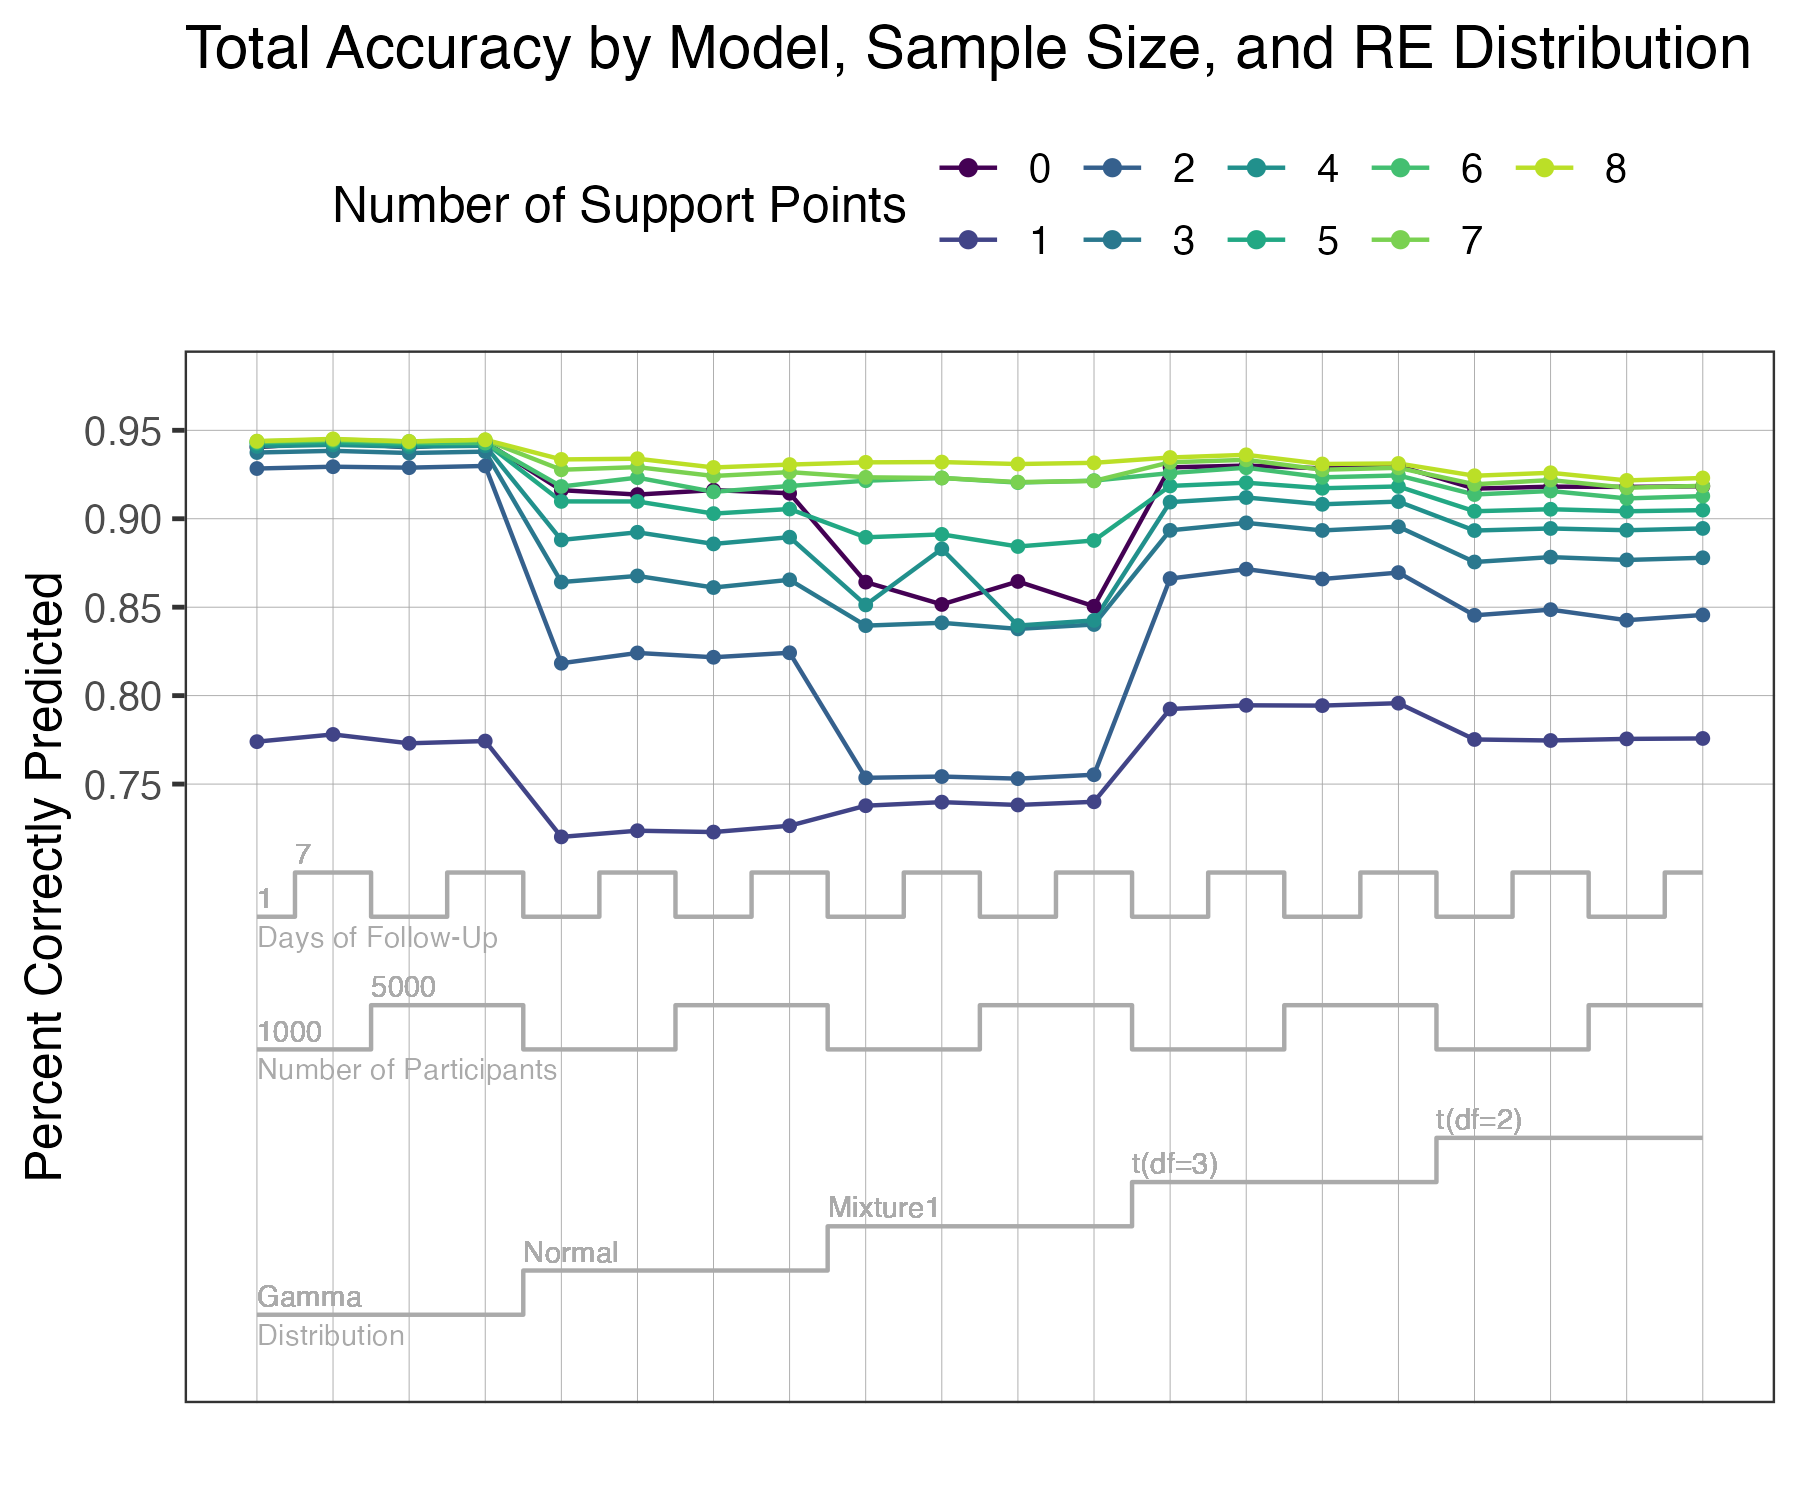
\includegraphics[scale=.8]{Support/NestedLoopAcc.png}
    \centering
    \caption{Nested loop plot of simulation results for total accuracy of predicted wake/sleep sequence. Each point is the median of 100 simulations. Color indicates model. The X axis indicates the simulation settings, which are a combination of days follow-up, number of participants, and RE distribution.}
    \label{NLacc}
\end{figure}
    
Figure \ref{NLacc} shows the results from the simulation in a nested loop (NL) plot. The y-axis for this figure is the accuracy of the estimated wake-sleep sequence compared to the true wake-sleep sequence. The color represents the model and the x-axis represents the different simulation settings. To read the NL plot, each point corresponds to a distinct combination of model and simulation settings. Take for example the left most light green point. On the x-axis, that point corresponds to simulated data with 1000 participants, 1 day of follow up, and where H is a Gamma distribution.

As can be seen from figure \ref{NLacc}, across all simulations the shared HMM and two support point MHMM have the lowest and second-lowest accuracy, respectively. Increasing the number of support points increases the accuracy, where a MHMM with 8 support points is the most accurate across all simulations. The increase in accuracy from each added support point diminishes, where H appears to determine both how quickly this increase diminishes and the maximum accuracy. For instance, when H is the Gamma distribution there is substantial gain from two to three support points, a marginal gain from three to four, and negligible gain from more than four. Overall, accuracy increases when the number of support points increases. The individual HMM performs well though this depends on H and the number of observations per person, performing similar to a MHMM with anywhere between four and eight support points. 
 




\begin{figure}
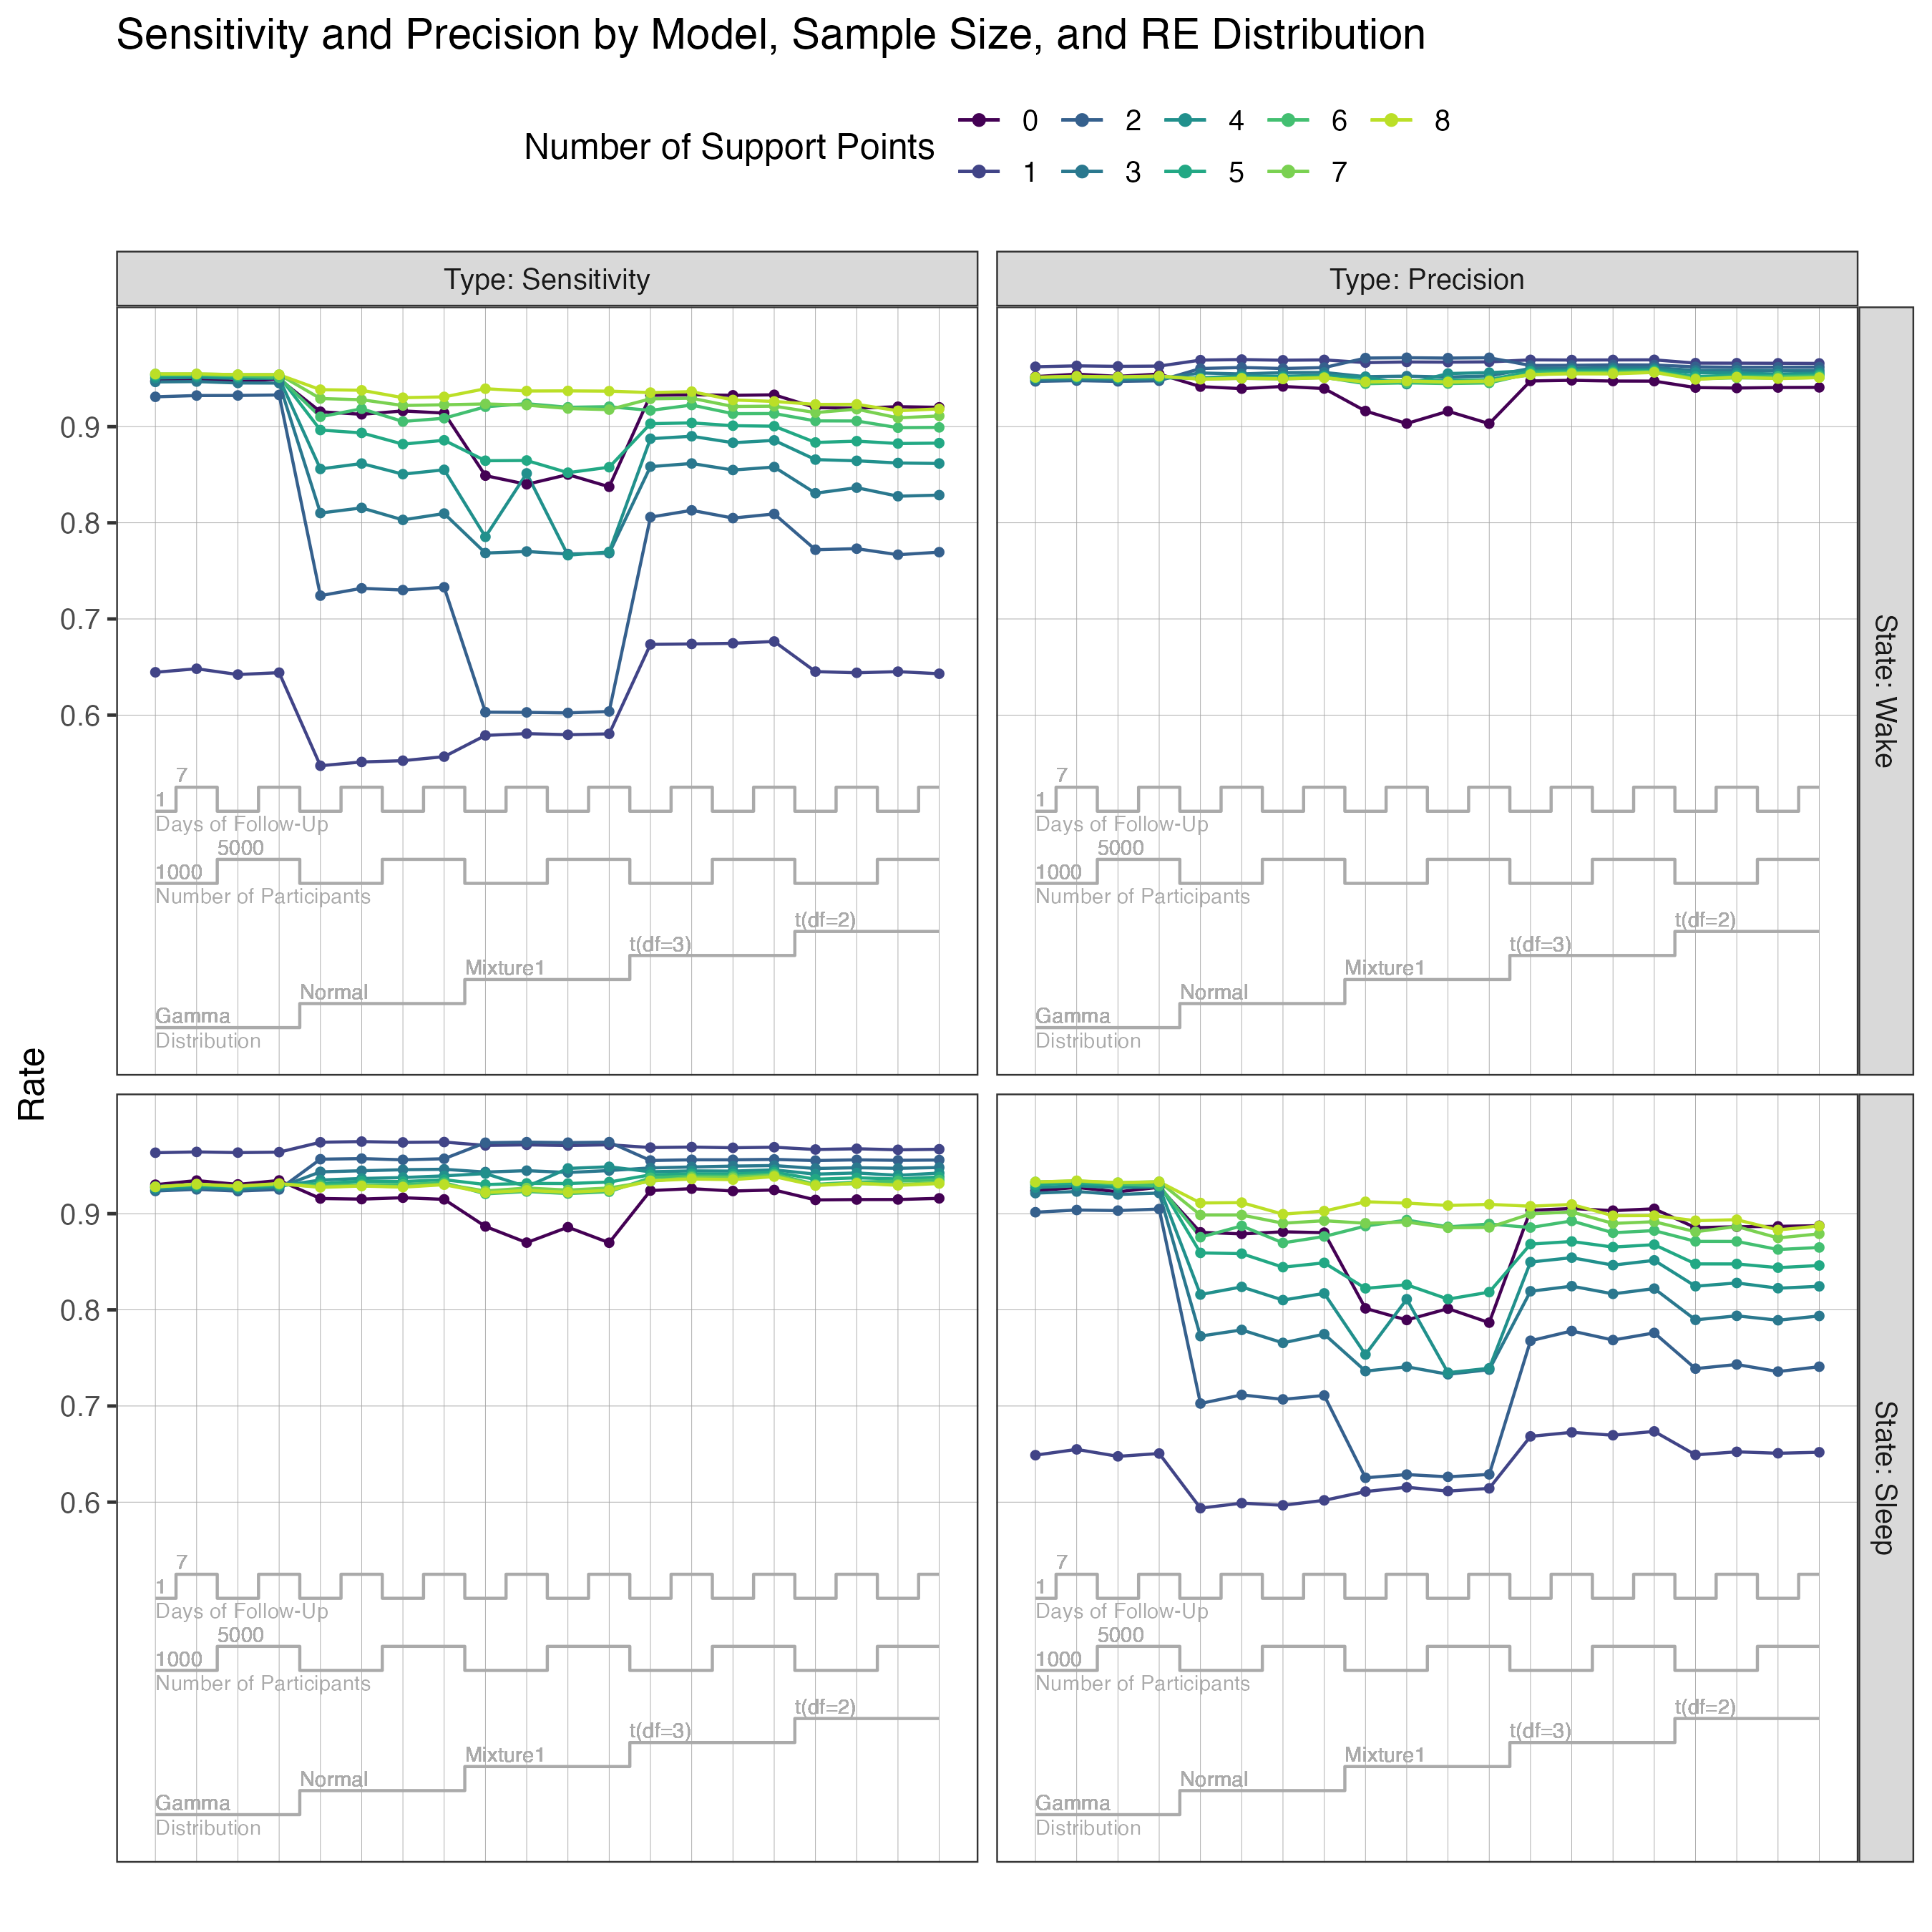
\includegraphics[scale=.65]{Support/NestedLoopSP.png}
\centering
\caption{Nested loop plot of simulation results for sensitivity (left column) and precision (right column) for wake (top row) and sleep (bottom row). Each point is the median of 100 simulations. Color indicates model used. The X axis indicates the simulation settings, which are a combination of days follow-up, number of participants, and RE distribution.}
\label{NL2}
\end{figure}

We examine the sensitivity and positive predictive value (PPV). Recall that wake sensitivity is the percent of all truly wake states that we accurately predict as wake, and wake PPV is the percent of predicted wake states that are truly wake. Figure \ref{NL2} shows the sensitivity (left column) and PPV (right column) for the wake (top row) and sleep (bottom row) states. Across all simulations the shared HMM and two support point MHMM has high sleep sensitivity, comparatively low wake sensitivity, and low sleep PPV. This indicates that in uncertain situations the models consistently predict the sleep state, even when the underlying state is wake. As the wake PPV is very high, the wake state is only predicted when it is clear that the underlying state is wake. When the number of support points is increased, the wake sensitivity increases, while the sleep sensitivity decreases slightly. This occurs because although we are better at predicting hard-to-classify wake behavior as wake, we also misclassify some sleep as wake, causing wake PPV to decrease and sleep PPV to increase. Similar to overall accuracy, the individual HMM performs similarly to a MHMM with somewhere between four and eight support points depending on the simulations settings.

\begin{figure}
    \includegraphics[scale=.65]{Support/NestedLoopTran.png}
    \centering
    \caption{Nested loop plot of simulation results for the 90th percentile of the absolute value of the transition residuals. The left column is the transition from sleep to wake and the right column is for wake to sleep. The rows are for the possible fixed covariates. Each point is the median of 100 simulations. Color indicates model used. X-axis indicates the simulation settings, which are a combination of days follow-up, number of participants, and RE distribution.}
    \label{NLtran}
\end{figure}

Increasing the number of support points also reduces the bias in the estimated transition matrix. Figure \ref{NLtran} is a NL plot for the $90^{\text{th}}$ percentile of the absolute value of the transition residuals across 100 simulations. As the transition probabilities are simulated as a first order harmonic, the absolute value of the residuals was chosen as it more accurately depicts the difference between the true and estimated probabilities compared to standard residuals. The left column is for the sleep to wake transitions and right for wake to sleep, and the rows are for each covariate grouping. Accurate state reconstruction occurs at the same number of support points as accurate transition probability estimation. This is in contrast to when the RE is in the transition process \cite{mcclintock2021}. Looking at the left half of figure \ref{NLtran}, the accuracy plateaus in figure \ref{NLacc} at the same number of support points where the transition residuals tend to zero. Similar to before, the bias of the individual HMM is dependent on both H and number of follow-up observations. Depending on the simulation settings, a MHMM clearly outperforms the individual HMM. Across all simulation settings, a MHMM with many (between five and eight) support points has the least amount of bias.

\begin{figure}
    \includegraphics[width=\textwidth]{Support/MiscParamBox.png}
    \centering
    \caption{Boxplot of $p_1$ (top left), $\sigma_0$ (top middle), $\mu_1$ (top right), $\sigma_1$ (bottom left), $\lambda_0$ (bottom middle), and $\lambda_1$ (bottom right) by model choice for 100 simulations with 1000 people, one day of follow up, and where H is a Gamma distribution. X-axis indicates model and Y axis is parameter estimate. The dashed horizontal line is the true parameter value.}
    \label{miscParam}
\end{figure}

Although accuracy might plateau, increasing the number of support points reduces the bias of other estimated parameters. Examining the 100 simulations for 1000 people with a day of follow up when H is a Gamma distribution, figure \ref{miscParam} contains information on the following estimated parameters: $p_1$ (top left), $\sigma_0$ (top right), $\mu_1$ (middle left), $\sigma_1$ (middle right), $\lambda_0$ (bottom left), and $\lambda_1$ (bottom right). Looking at the plot for $\sigma_0$, although the accuracy might remain somewhat constant when the number of support points is increased beyond three, the wake standard error bias continually decreases. Even with eight support points there is a small amount of bias. In contrast, the individual HMM is not biased when estimating $\sigma_0$, however it is when estimating the sleep emission parameters. 

\begin{figure}
    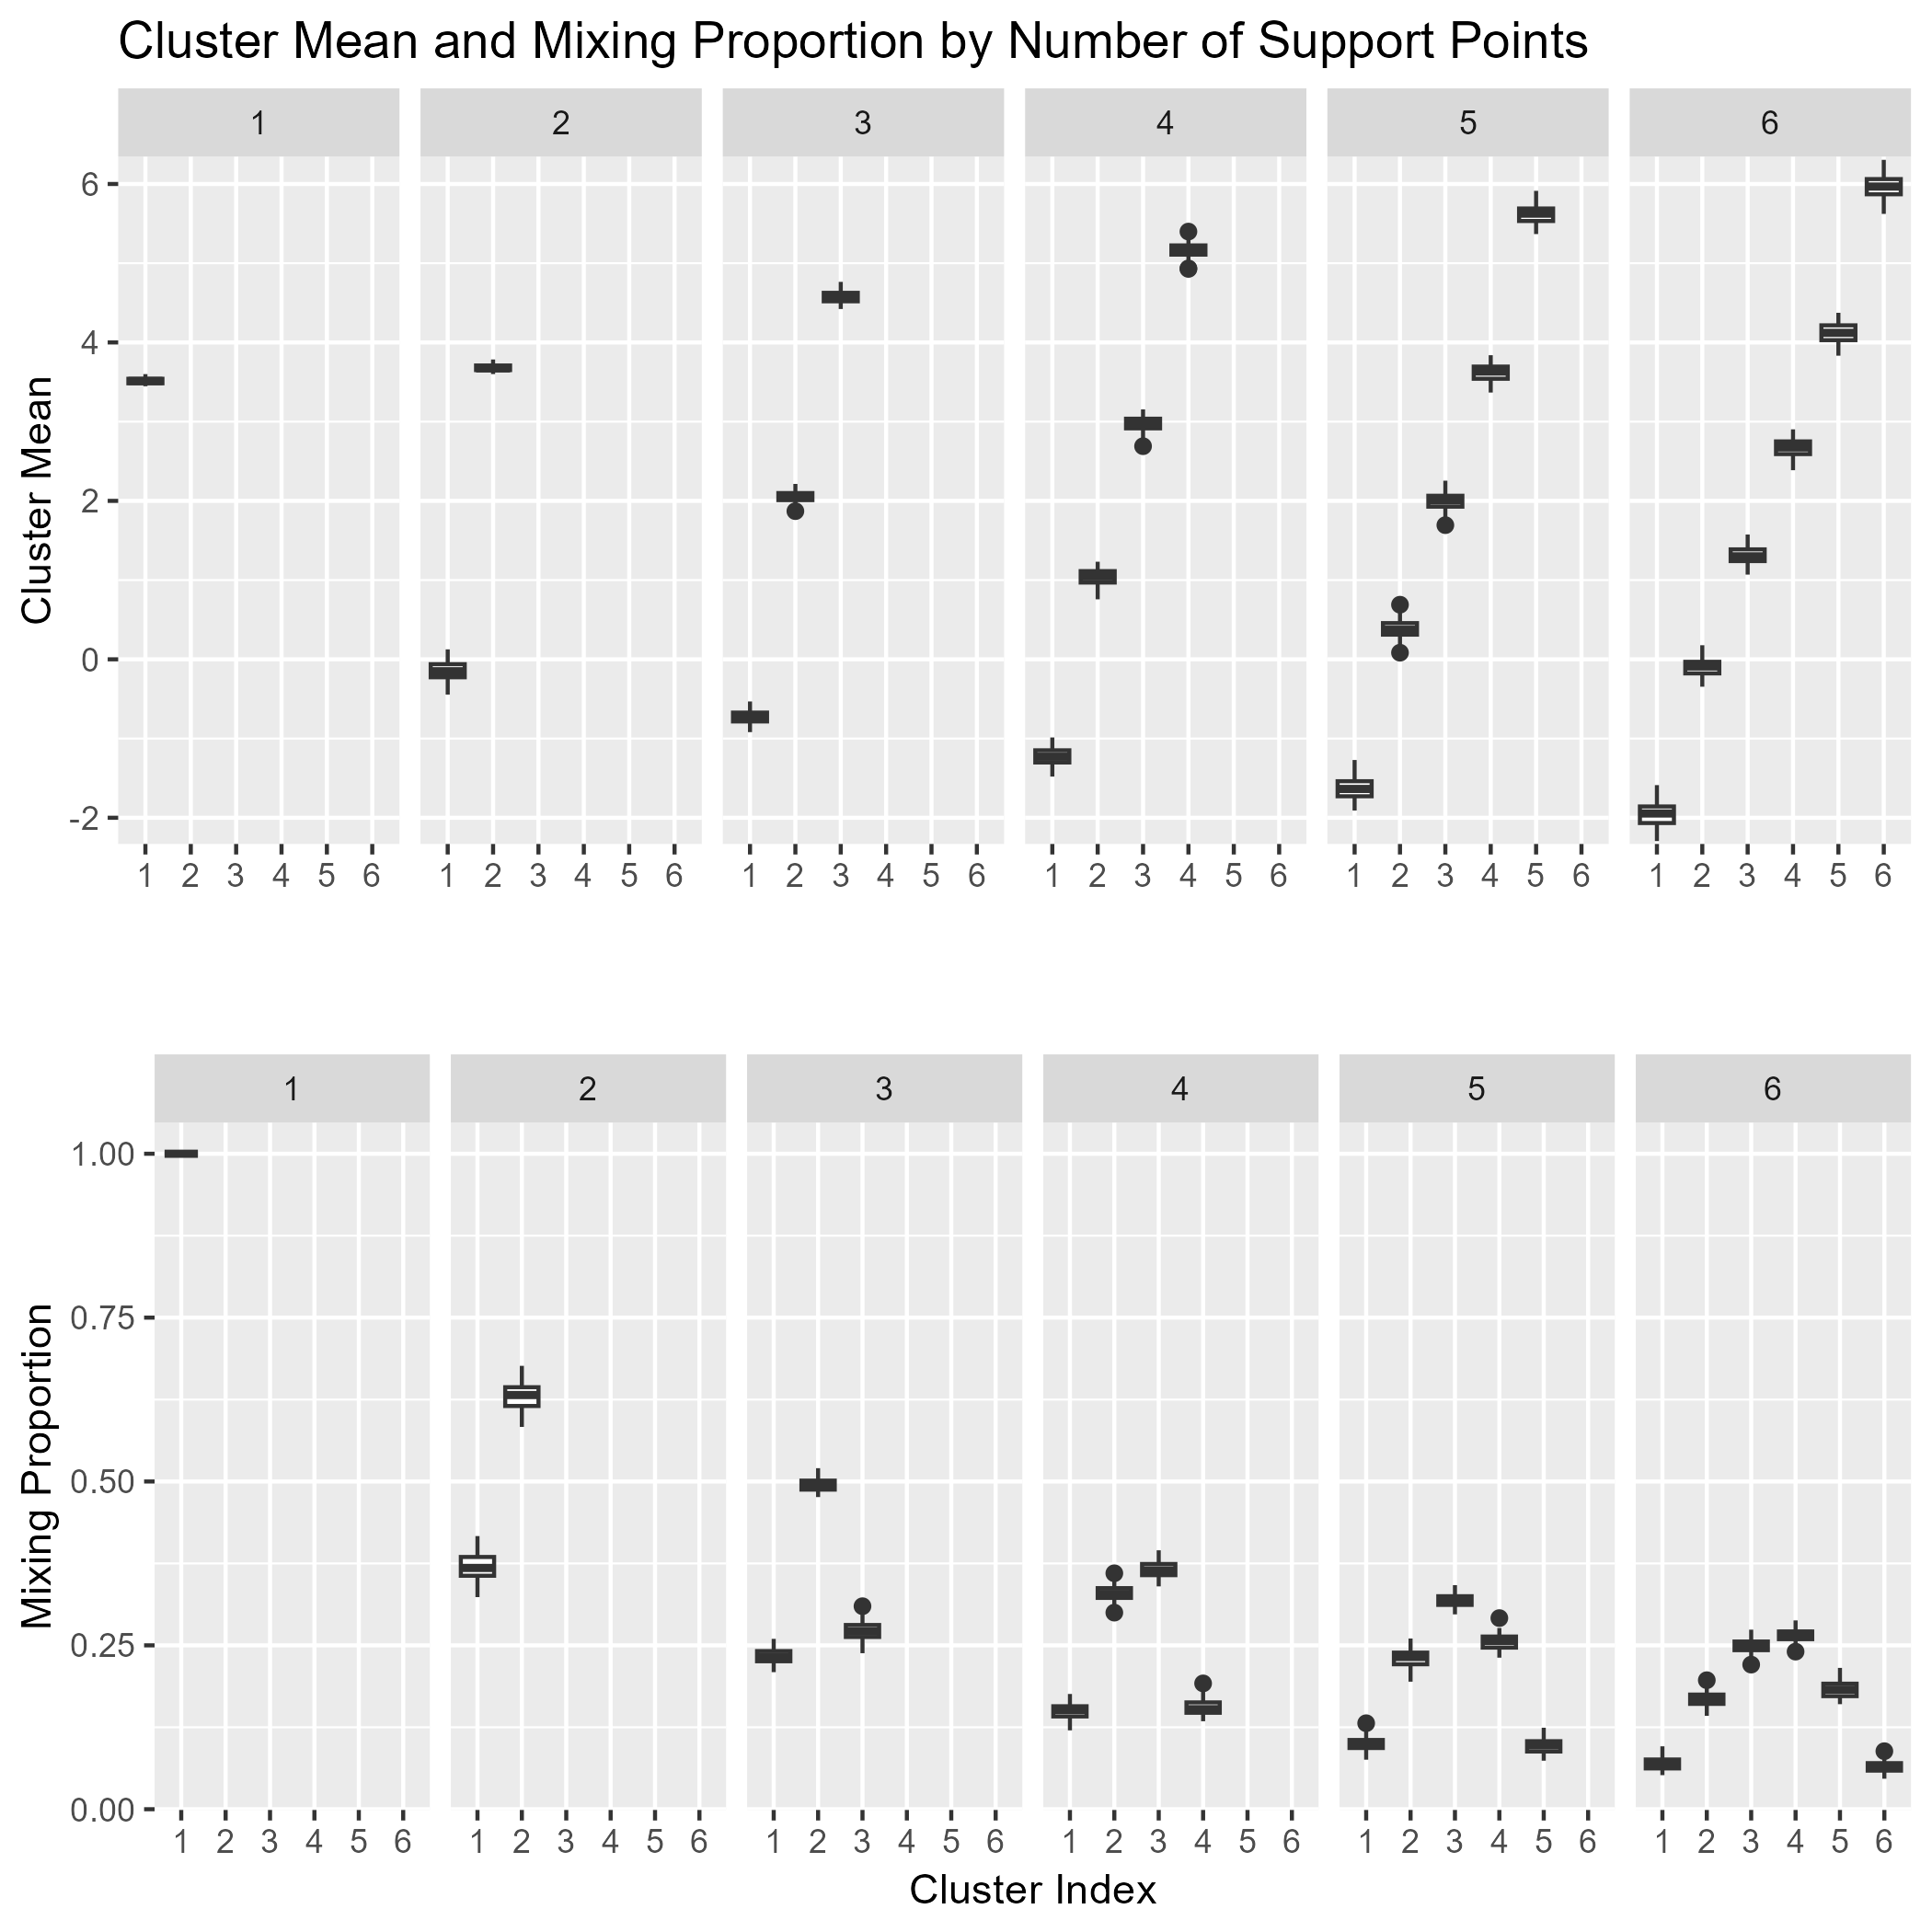
\includegraphics[scale=.48]{Support/clustmeanmix.png}
    \centering
    \caption{Scatter plot of mixing proportion ($\pi_l$) by cluster mean ($\nu_l = \mu_0+r_l$) for a MHMM with one through eight support points. Each point represents the median of 100 simulations with 1000 people, one day of follow up, and where H is a Gamma distribution.}
    \label{CMM}
\end{figure}

Continuing with the same Gamma simulation, we can get a better sense of how increasing the number of support points increases overall accuracy and reduces bias by looking at figure \ref{CMM}, which plots the mixing proportion $(\pi_l)$ against the cluster mean $(\hat{\nu_l})$. Each gray box indicates the number of support points used in the MHMM. With one support point (which is equivalent to the shared HMM) we have a cluster at around 3.5 and roughly 55\% accuracy. Using two support points we have clusters at around 1.75 and 4.25 and an accuracy of 80\%. With three support points we have clusters at around 0, 2.75 and 5.25 and an accuracy of 90\%. These new clusters closer to 0, and thus closer to the mean sleep activity, help accurately predict wake when we observe low activity generated by a wake state. As the number of support points increases, a Gamma distribution takes shape in figure \ref{CMM}, however after four support points the accuracy gains are negligible.

\begin{figure}
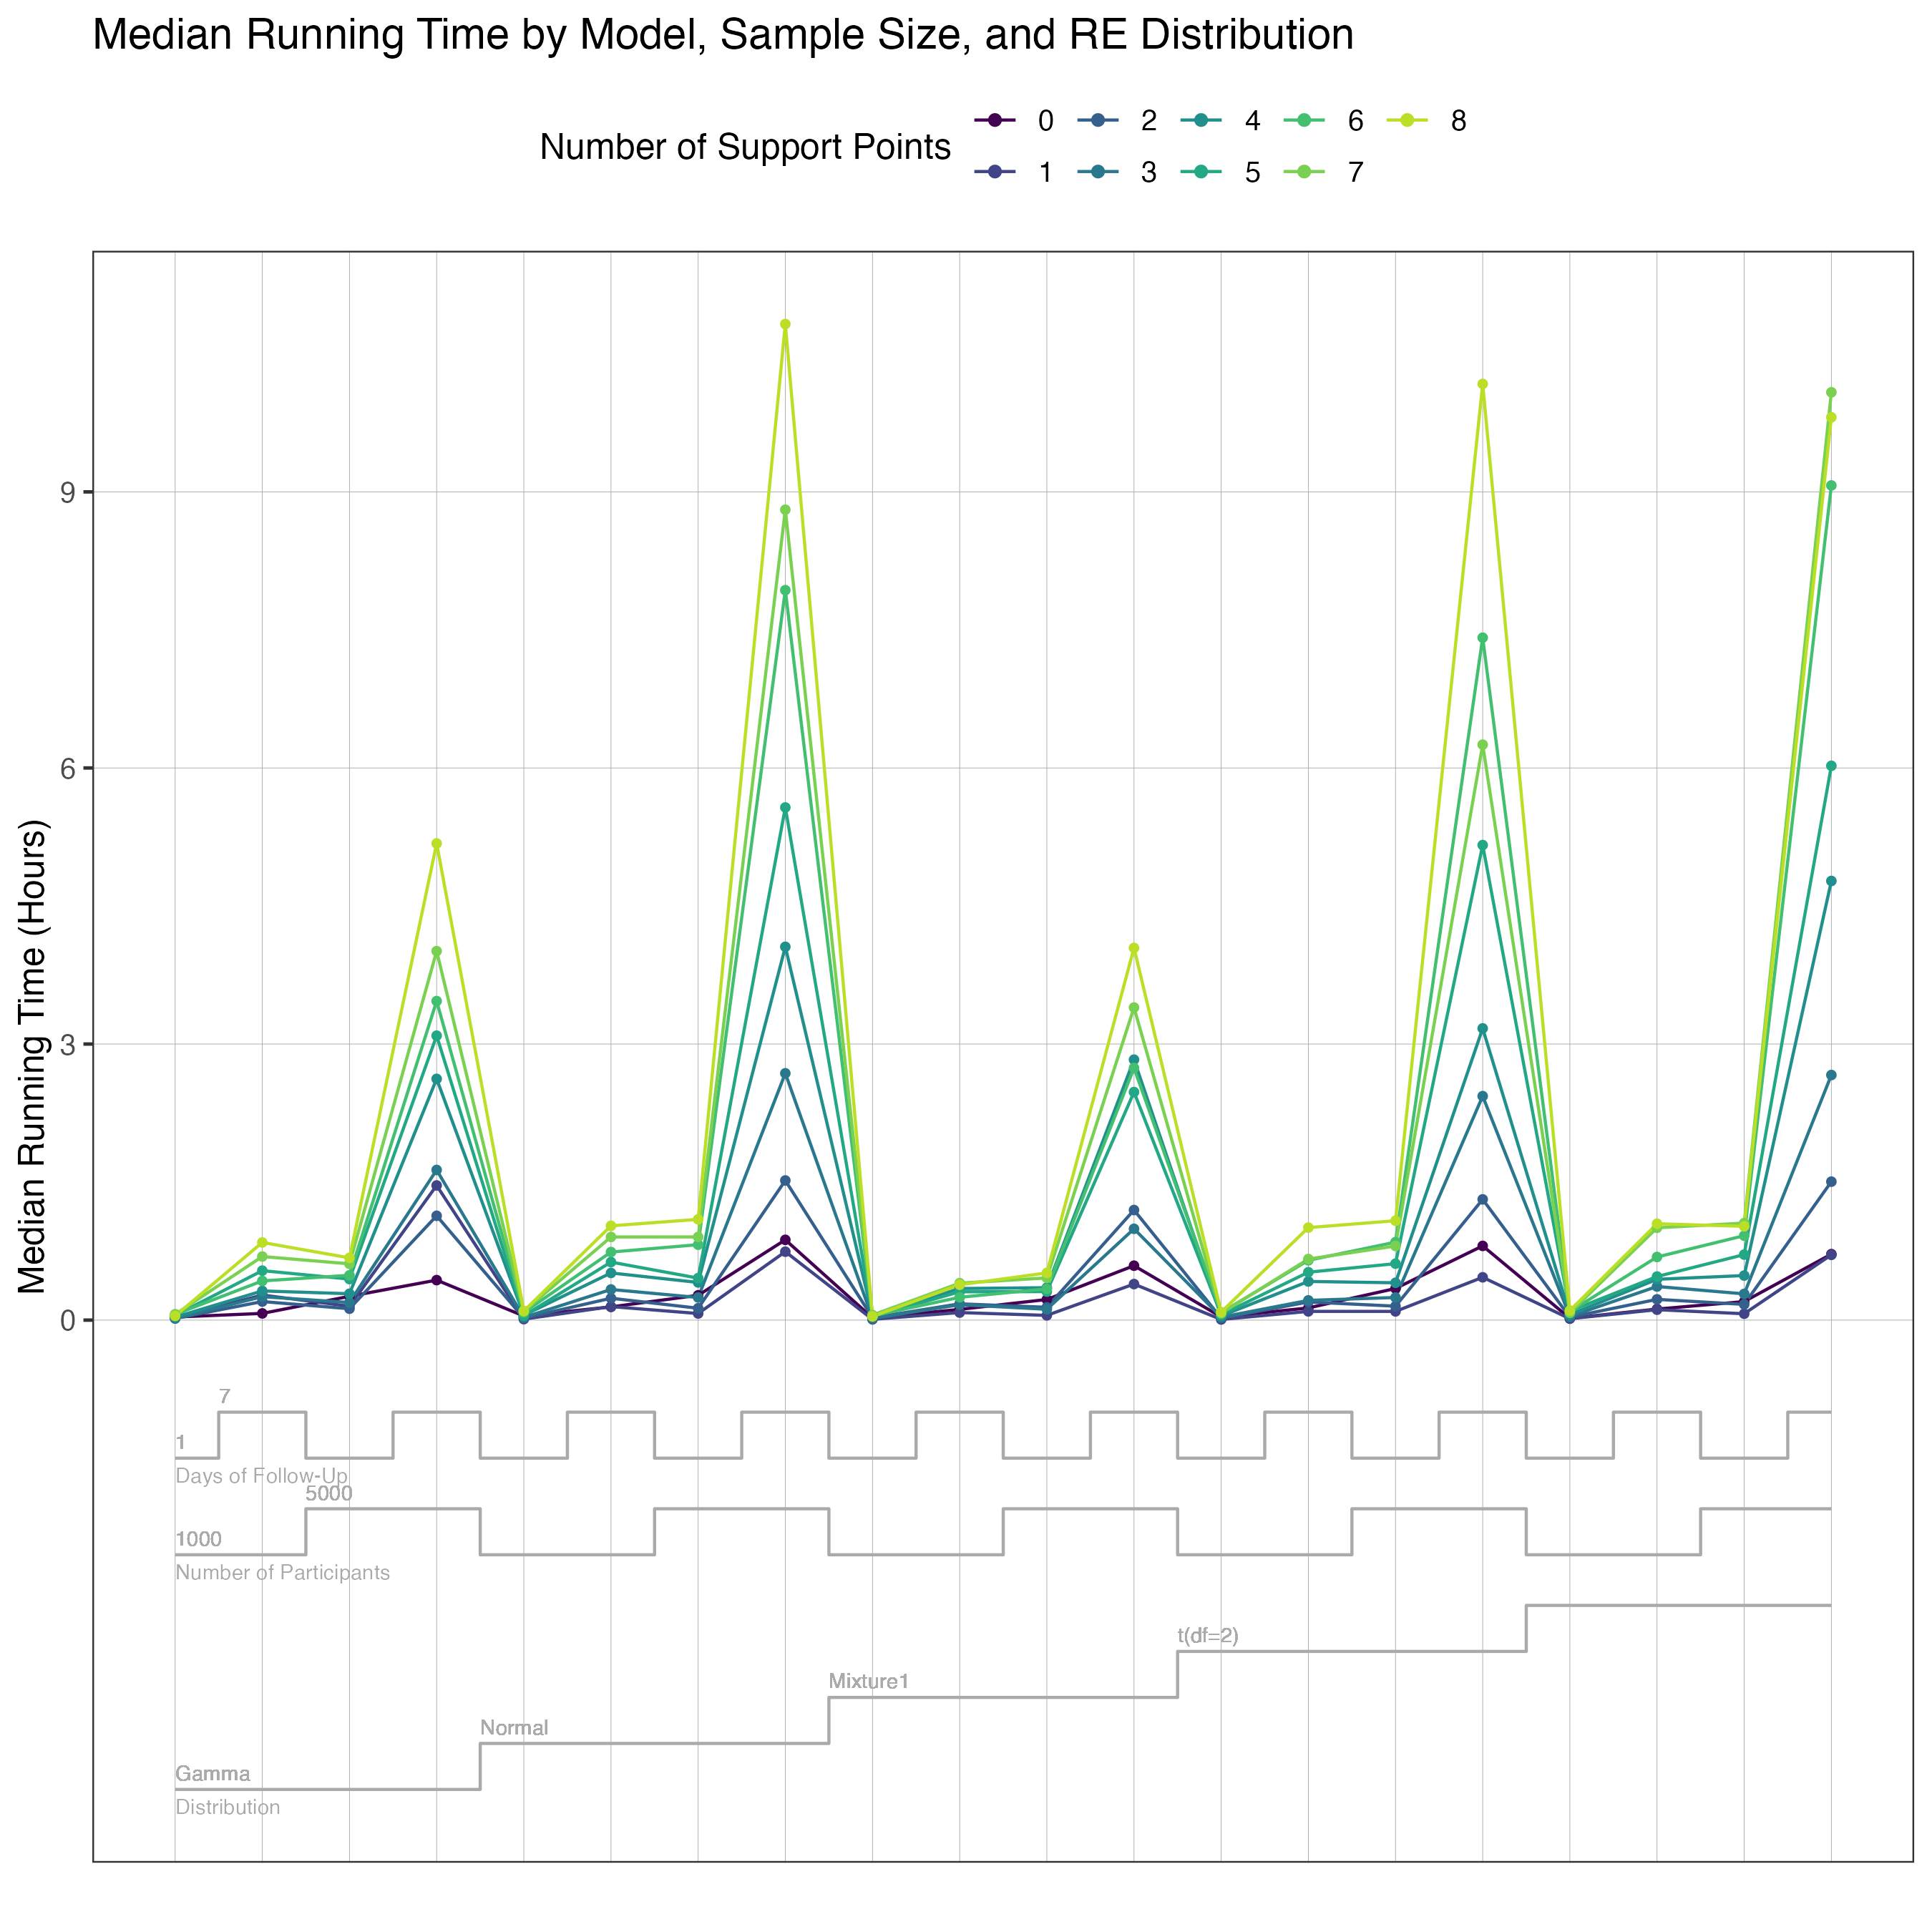
\includegraphics[scale=.4]{Support/NestedLoopCompTime.png}
\centering
\caption{Nested loop plot of simulation results for median run time in hours. Each point is the median of 100 simulations. Color indicates model used. X-axis indicates simulation settings, which is a combination of days follow-up, number of participants, and RE distribution.}
\label{time}
\end{figure}

Figure \ref{time} is a NL plot showing the median run time in hours. We see that the increasing the number of support points generally increases the median run time. For all the simulations barring the t distribution with three degrees of freedom, three to six support points is sufficient for maximum accuracy. For a t distribution with three degrees of freedom it may be beneficial to use eight support points, despite the increased time. Unlike for heterogeneity in the hidden process, where high accuracy does not necessarily indicate unbiased parameters \cite{mcclintock2021}, when the accuracy plateaus the parameter estimates are minimally biased (except $\sigma_0$).


\subsection{Discussion}\label{SimStudyDiscussion}

Standard HMMs are often faster and easier to implement, however MHMMs may provide higher accuracy given a sufficient number of support points are chosen. Increasing the number of support points reduces bias and improves latent state prediction, however it also increases model run time. In many of the previous simulations, the individual HMM performs similar to the MHMM. The individual HMM is flexible and is able to capture minute differences in activity between people, however, it has a number of key drawbacks. Many repeated measurements are needed per person to estimate each mean parameter. For instance the model was less accurate and more biased when analyzing one day of follow up compared to the one week of follow up. Additionally, overall accuracy depends on the underlying RE distribution H, which is unlikely to be known. Although the individual wake activity parameters allow for flexible modeling, the number of parameters increases with the number of people.

BIC has previously been proposed for HMM and MHMM model selection \cite{maruotti2009}. We have found that in simulations with one day of follow up the MHMM with 8 support points has the lowest BIC. For one week of follow, up either the MHMM with eight support points or the individual HMM has the lowest BIC, depending on H. If there are many observations per person or minimizing algorithm run-time is important, an individual HMM may be better suited than a MHMM. For situations with relatively few observations per person or in settings where consistent accuracy irrespective of the underlying RE distribution is paramount, MHMMs may be preferred. 

As the number of necessary support points appears to depend on H, choosing the number of support points will depend on the overall goal of the model. If state reconstruction or transition probability estimation is the primary goal, then successive MHMMs can be run increasing the number of support points by 1 until the reconstructed sequence is similar between models. If estimation of emission related parameters is more important, then BIC can be used to decide.  

Increasing the number of support points increases the accuracy of the state reconstruction and reduces bias, however there are diminishing returns. As the necessary run time roughly scales linearly with the number of support points, it is pertinent that we choose enough support points to accurately estimate the sequence without significant computational burden. 

\section{Application}

The National Health Examination Survey (NHANES) is a collection of studies aiming to quantify the health of US civilians. Beginning in 1960, NHANES became a yearly study in 1999 where specific goals change year-to-year to focus on emerging issues. For the 2011-2012 and 2013-2014 waves, a representative sample of the US were given a wrist physical activity monitor (PAM) for 9 days. Among other metrics, these PAMs measured physical activity by the minute. This data offers a unique glimpse into the circadian rhythm for the US population.

For the 2011-2012 and 2013-2014 waves, participants were given an ActiGraph (model GT3X+) for nine days which measured triaxial movement summaries by the minute in open source MIMS units \cite{Dinesh2019}. Minute data was removed (as if missing) when a quality flag was present, triaxial movement was negative, or the PAXPRED variable predicted non-wear. The median of each 15-minute period was used to reduce the computational burden. Sample weights were included in the likelihood \cite{Karchin1998} to account for the complex sample design. 

HMMs for actigraphy data are typically run on each individual separately. Although this can account for person-to-person variability, this approach would not be able to incorporate the necessary NHANES sample weights. Our models run on all individuals at once and allow for heterogeneity in both the emission distribution and the state transition process. Different levels of wake activity are allowed described by section \ref{Methods}. Age is included as a covariate in the transition probabilities as it has shown to be an important factor impacting sleep \cite{Redline2004,Boselli1998}. Age has been discretized into the following six categories: less than 11, 11-20, 21-35, 36-50, 51-65, greater than 65. Additionally, we included harmonic terms in the transition calculations to account for the cyclical nature of the circadian rhythm. As NHANES is a nationally representative sample, by running the models on the population as a whole we can calculate HMM parameters for the entire sample. 

We applied both the individual HMM and MHMM with eight support points to NHANES actigraphy data to illustrate the differences (or lack thereof) in the models. The MHMM with eight support points was chosen as it had the lowest BIC of all MHMMs fit. After estimation the Viterbi algorithm was used to predict the most likely sequence of wake/sleep states. As we do not have access to the same information often included in sleep studies (e.g., time spent in bed), alternative metrics must be used. From the Viterbi sequence we can calculate the following sleep summary measures: longest sleep block, time of sleep onset, sleep efficiency, and daily total sleep \cite{Su2022}. The longest sleep block was calculated as the longest block of sleep from 12:00pm to 12:00pm on the following day that was interrupted by no more than a continuous 1.5 hours of wake. Time of onset is defined as the start time of the longest sleep block. Sleep efficiency is defined as the percent of time sleeping during the longest sleep block. Daily total sleep time is defined as the total amount of sleep between 12:00pm and 12:00pm on the following day.

\subsection{Results and Discussion}

\begin{figure}
    \includegraphics[width=.9\textwidth]{Support/RealSleepSumPlot.png}
    \centering
    \caption{Sleep summary statistics for the individual HMM and MHMM with eight support points by age or BMI. Sleep onset is defined as the start of the longest sleep block and sleep efficiency is the percent of time asleep during the longest sleep block. The longest sleep block is the longest block of sleep interrupted by no more than 1.5 hours of continuous wake.}
    \label{SleepSum}
\end{figure}

We examined time of sleep onset, sleep efficiency, and total sleep by plotting the summary statistics against age, BMI, ratio of household income to poverty line, race, and gender. We see in figure \ref{SleepSum} that sleep onset is early when young, peaks at around age 20 and then decreases with age. Daily total sleep is high when young, decreases and remains fairly constant from 20-40, and then increases afterwards. Sleep efficiency is high when young and starts to gradually decrease after around 20 years old. These findings are consistent with previous research \cite{Su2022}. We found that sleep efficiency is lower for people with higher BMIs. The results for sleep onset and daily total sleep are very similar between the individual HMM and the MHMM with eight support points. For sleep efficiency, the MHMM estimated lower values, however the overall trend is still similar. There did not appear to be any relationship between the sleep metrics and the remaining sociodemographic variables. 

\begin{figure}
    \includegraphics[width=.8\textwidth]{Support/AgeBMIClustDensity.png}
    \centering
    \caption{Density of age and BMI by cluster for a MHMM with eight support points. Clusters are ordered by increasing mean activity starting with cluster one.}
    \label{AgeBMIdens}
\end{figure}


Despite a lower BIC compared to the individual HMM, one benefit of the MHMM is that it implicitly clusters heterogeneity in the emission distribution. Figure \ref{AgeBMIdens} shows the density of BMI and age for each of the 8 clusters from the MHMM with eight support points. The clusters are ordered such that cluster one has the lowest activity and eight the highest. We see that lower activity clusters are older with a higher BMI while the more active clusters are younger with a lower BMI. This is an unsupervised clustering based on activity that is incorporated into the model estimation. This clustering is distinct from a k-means clustering of the mean wake activity parameters from the individual HMM, which favors smaller, more distant clusters. Figure \ref{CMMreal} is analogous to figure \ref{CMM}, but for the NHANES data and gives a sense of the estimated mean activity distribution. It is roughly symmetrical with a mean at around 2.5 and a long left tail. This tail indicates that there are some people who are particularly sedentary. 

\begin{figure}
    \includegraphics[width=.8\textwidth]{Support/CMMreal.png}
    \centering
    \caption{Scatter plot of mixing proportion ($\pi_l$) by cluster mean ($\nu_l$) for a MHMM with one through eight support points run on the NHANES dataset.}
    \label{CMMreal}
\end{figure}

As a sensitivity analysis we have fit the models using BMI (less than 18.5, 18.5-25, 25-30, 30-35, 35-40, greater than 40) and household income ratio to the poverty line (0-1, 1-2, 2-3, 3-4, 4-5, greater than 5) as the covariates in the transition process with similar results. Additionally, we adjusted the longest sleep block calculation by increasing the amount of continuous wake allowed from 1.5 to three hours with minimal change. 


\section{Conclusion}


Despite the much smaller number of parameters, in simulations a MHMM performs similarly or better than the individual HMM depending on the number of support points. MHMMs do not require as many repeated measurements per person to be accurate and require fewer estimated parameters. MHMMs also naturally cluster the data and therefore are very interpretable when examining heterogeneity in a population. However, MHMMs are not without their drawbacks. HMMs are much easier to implement as one can rely on off-the-shelf packages. There is a trade-off between accuracy and computational time that must be balanced as standard HMMs are much faster, especially for large amounts of data. 

As state reconstruction is often the goal when applying HMMs to actigraphy data, a MHMM may be preferred over an individual HMM when the length of time is relatively short (such as analyzing weekend only data). Additionally, if the goal is to characterize the heterogeneity of the population, MHMMs cluster the data in an interpretable way.  However, as most actigraphy applications have long follow-up lengths, standard HMMs provide similar levels of accuracy with shorter run times and easier implementations. 

\bibliographystyle{unsrtnat}
\bibliography{Support/MHMMbib}

\end{document}
